\documentclass{article}

\usepackage{fancyhdr}
\usepackage{extramarks}
\usepackage{amsmath}
\usepackage{amsthm}
\usepackage{amsfonts}
\usepackage{tikz}
\usepackage{graphicx} %插入图片的宏包
\usepackage{float} %设置图片浮动位置的宏包
\usepackage{pythonhighlight}
% \usepackage{subfigure} %插入多图时用子图显示的宏包
% \usepackage[plain]{algorithm}
% \usepackage{algpseudocode}

% \usetikzlibrary{automata,positioning}

%
% Basic Document Settings
%

\topmargin=-0.45in
\evensidemargin=0in
\oddsidemargin=0in
\textwidth=6.5in
\textheight=9.0in
\headsep=0.25in

\linespread{1.1}

\pagestyle{fancy}
\lhead{\hmwkAuthorName}
\chead{\hmwkClass\ : \hmwkTitle}
\rhead{\firstxmark}
\lfoot{\lastxmark}
\cfoot{\thepage}

\renewcommand\headrulewidth{0.4pt}
\renewcommand\footrulewidth{0.4pt}

\setlength\parindent{0pt}


%代码格式设置



%
% Create Problem Sections
%

\newcommand{\enterProblemHeader}[1]{
    \nobreak\extramarks{}{Problem \arabic{#1} continued on next page\ldots}\nobreak{}
    \nobreak\extramarks{Problem \arabic{#1} (continued)}{Problem \arabic{#1} continued on next page\ldots}\nobreak{}
}

\newcommand{\exitProblemHeader}[1]{
    \nobreak\extramarks{Problem \arabic{#1} (continued)}{Problem \arabic{#1} continued on next page\ldots}\nobreak{}
    \stepcounter{#1}
    \nobreak\extramarks{Problem \arabic{#1}}{}\nobreak{}
}

\setcounter{secnumdepth}{0}
\newcounter{partCounter}
\newcounter{homeworkProblemCounter}
\setcounter{homeworkProblemCounter}{1}
\nobreak\extramarks{Problem \arabic{homeworkProblemCounter}}{}\nobreak{}

%
% Homework Problem Environment
%
% This environment takes an optional argument. When given, it will adjust the
% problem counter. This is useful for when the problems given for your
% assignment aren't sequential. See the last 3 problems of this template for an
% example.
%
\newenvironment{homeworkProblem}[1][-1]{
    \ifnum#1>0
        \setcounter{homeworkProblemCounter}{#1}
    \fi
    \section{Problem \arabic{homeworkProblemCounter}}
    \setcounter{partCounter}{1}
    \enterProblemHeader{homeworkProblemCounter}
}{
    \exitProblemHeader{homeworkProblemCounter}
}

%
% Homework Details
%   - Title
%   - Due date
%   - Class
%   - Section/Time
%   - Instructor
%   - Author
%

\newcommand{\hmwkTitle}{Quiz\ \#8}
\newcommand{\hmwkDueDate}{Jan 9, 2019}
\newcommand{\hmwkClass}{Complex Networks}
\newcommand{\hmwkClassTime}{Section A}
% \newcommand{\hmwkClassInstructor}{Professor Isaac Newton}
\newcommand{\hmwkAuthorName}{\textbf{RUOPENG XU} }
\newcommand{\hmwkAuthorNum}{\textbf{18M38179} }

%
% Title Page
%

\title{
    \vspace{2in}
    \textmd{\textbf{\hmwkClass:\ \hmwkTitle}}\\
    \normalsize\vspace{0.1in}\small{Due\ on\ \hmwkDueDate\ }\\
    % \vspace{0.1in}\large{\textit{\hmwkClassInstructor\ \hmwkClassTime}}
    \vspace{3in}
}

\author{\hmwkAuthorName\\ \hmwkAuthorNum}
\date{}

\renewcommand{\part}[1]{\textbf{\large Part \Alph{partCounter}}\stepcounter{partCounter}\\}

%
% Various Helper Commands
%

% Useful for algorithms
\newcommand{\alg}[1]{\textsc{\bfseries \footnotesize #1}}

% For derivatives
\newcommand{\deriv}[1]{\frac{\mathrm{d}}{\mathrm{d}x} (#1)}

% For partial derivatives
\newcommand{\pderiv}[2]{\frac{\partial}{\partial #1} (#2)}

% Integral dx
\newcommand{\dx}{\mathrm{d}x}

% Alias for the Solution section header
\newcommand{\solution}{\textbf{\large Solution}}

% Probability commands: Expectation, Variance, Covariance, Bias
\newcommand{\E}{\mathrm{E}}
\newcommand{\Var}{\mathrm{Var}}
\newcommand{\Cov}{\mathrm{Cov}}
\newcommand{\Bias}{\mathrm{Bias}}

\begin{document}

\maketitle

\pagebreak

\begin{homeworkProblem}
    % questions
 Make a program of breadth‐first search (BFS).

% 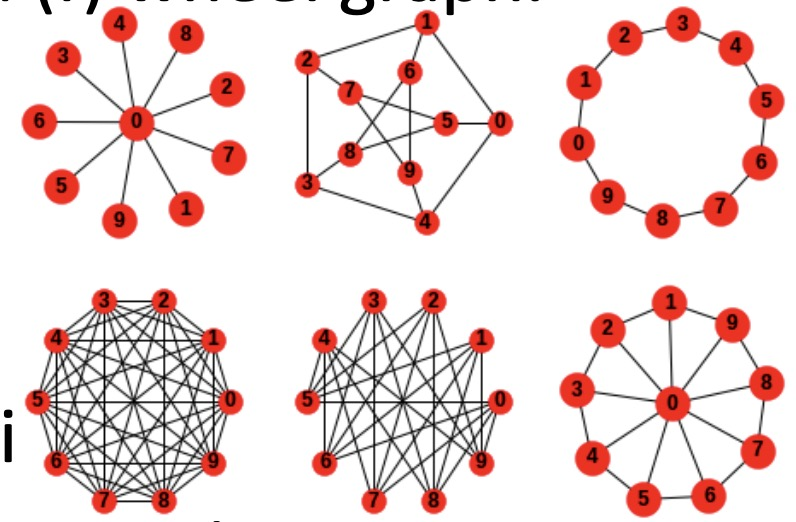
\includegraphics[scale=0.3]{quiz6_1.jpg}

\subsection*{Answer 1}
The BFS made by myself:
\begin{python}
import networkx as nx

# note the iterated nodes as 1
# push the current node into list2(FIFO) 
# -> push its adjanct nodes into list2 
# ->dequeue current node

def my_BFS(G,s):
    count = 0
    statement = []
    queue = []
    n = len(G)
    result = []
    
    # use one list to save the statement
    # initial all nodes as zero (haven't iterate)
    for node in range(0,n):
        statement.append(0)
        
    #visit the source node         
    queue.append(s)
    count = count + 1
    statement[s] = 1
  
    
    
    while(queue!=[]):
        current = queue[0]
        result.append(current)
        
        #if haven't reach the node, push it into the queue
        if(count-1<n):
            for i in G[count-1]:
                if(statement[i] == 0):
                    queue.append(i)
                    
        # dequeue current node
        queue.remove(current)
        count = count + 1
        
        #change the statement of nodes in queue
        for v in queue:
            statement[v] = 1
    return result
            
G = nx.karate_club_graph()
source = 0
result = my_BFS(G,source)
print(result)
\end{python}
and the result is:
\begin{python}
[0, 1, 2, 3, 4, 5, 6, 7, 8, 10, 11, 12, 13, 17, 19, 21, 31, 30, 9, 27, 28, 32, 16, 33, 25, 29, 23, 24]
\end{python}


\end{homeworkProblem}
\pagebreak


\begin{homeworkProblem}
Show the final status of distance array and queue after
BFS is done from vertex 0 of Karate club network.
\subsection*{Answer 2}
After BFS has been done, the queue is empty.
\\
\\
Ths distance array is:
\\
$[0, 1, 1, 1, 1, 1, 1, 1, 1, 2, 1, 1, 1, 1, 3, 3, 2, 1, 3, 1, 3, 1, 3, 3, 2, 2, 3, 2, 2, 3, 2, 1, 2, 2]$
\end{homeworkProblem}
\pagebreak


\begin{homeworkProblem}
Explain why BFS is not good for networks with varying
edge lengths.
\subsection*{Answer 3}
In BFS, it will search all of the nearest nodes from the source firstly, and after that expand the nodes connected to the current node. So the depth of searching is small and need a lot of memory to storage the array.
\\
If the edge length is varying, which means the graph is deeper, BFS may not have a good performance because of the huge cost of space. In terms of mathematics, the space complexity of BFS is O($B^{M}$)(\textit{from wiki}), in which B is the max number of branches and M is the max length of the tree. Therefore, with more branches and when the graph is deeper, the space cost will increase.
\end{homeworkProblem}
\pagebreak

\end{document}
%
% Non sequential homework problems
%

% Jump to problem 18
